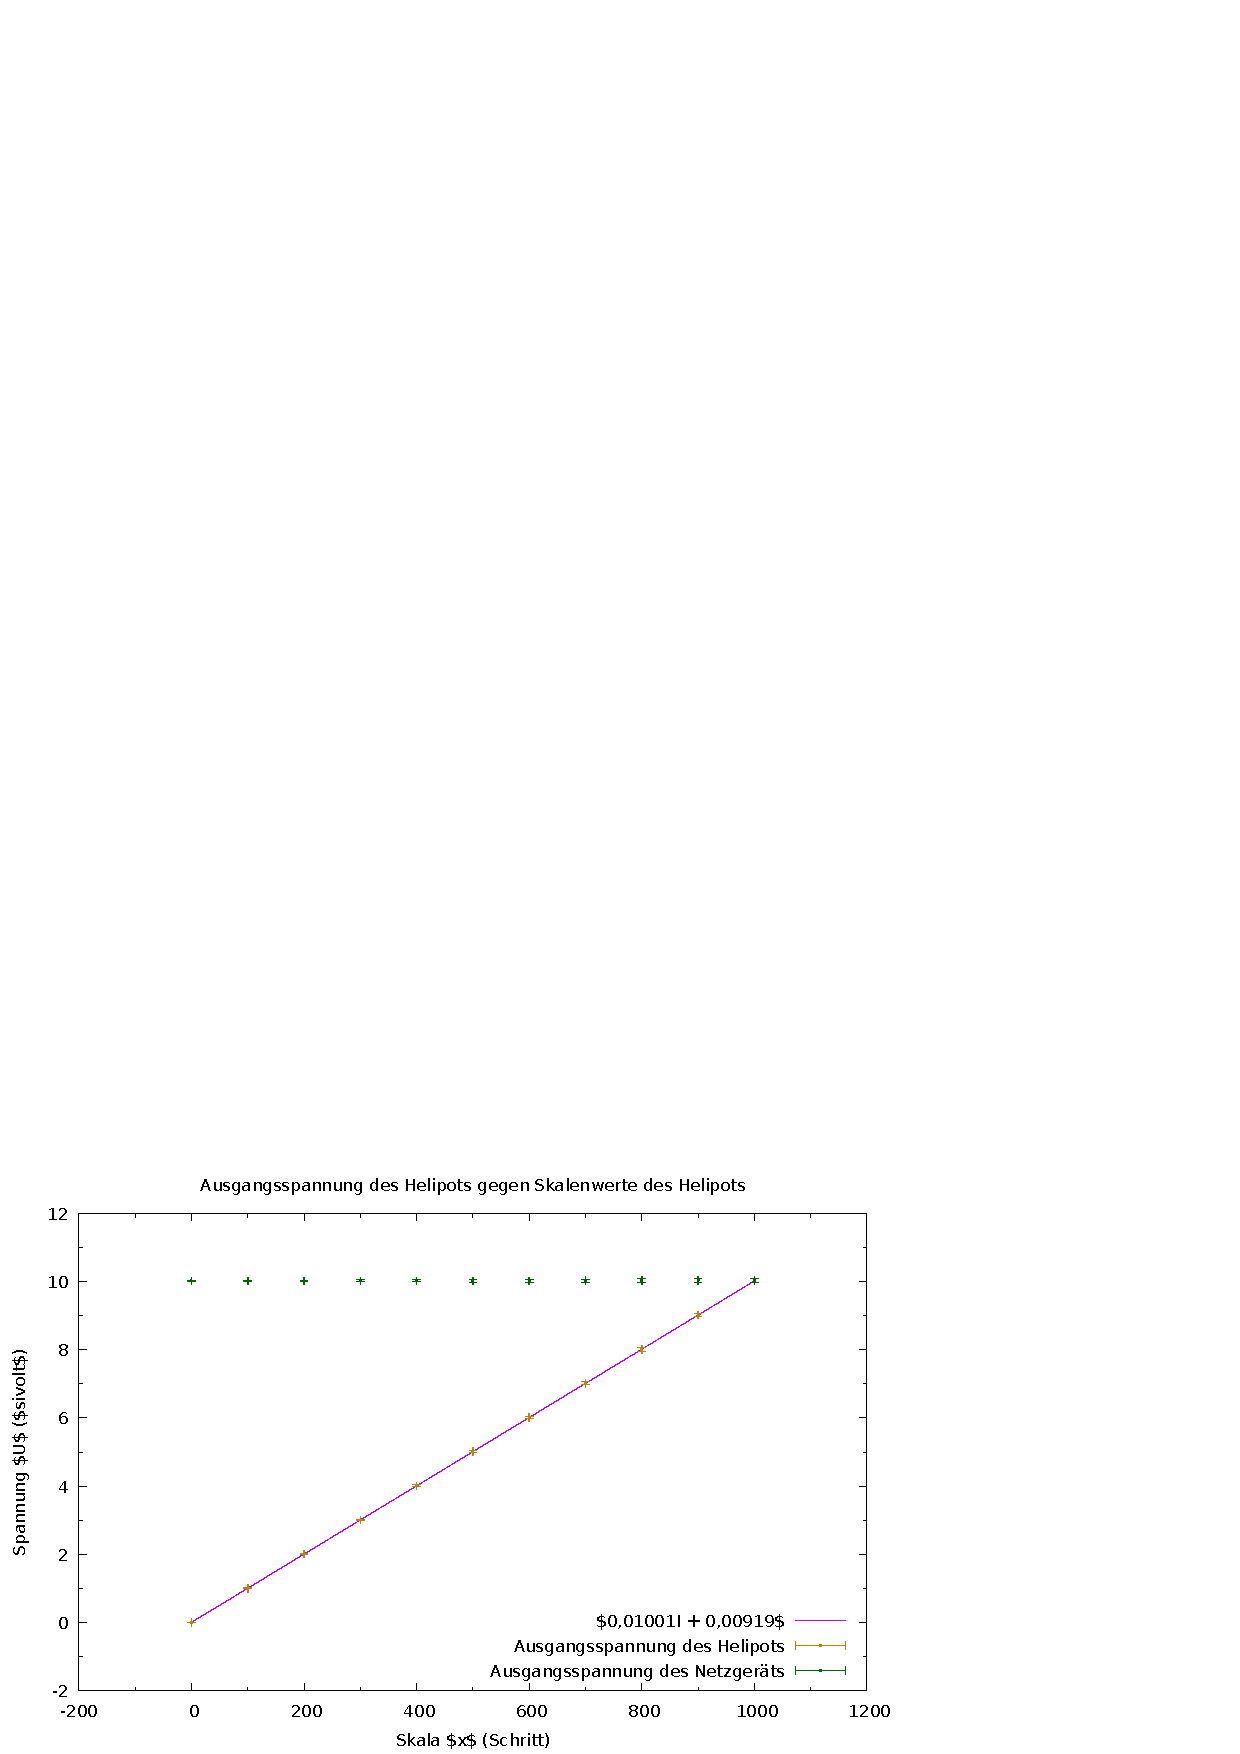
\includepdf{./scans/tv3.pdf}
\section{Teilversuch 3: Induktion durch Drehen einer Spule in einem Magnetfeld}
	Die Amplitude $U_0$ sind von der Graph gelesen und wir erhalten als Messwerten:
	\begin{equation*}
		\begin{tabu}{l *{9}{r}}
			\toprule
			U_0 / \si{\volt} & 1,040 & 1,040 & 1,065 & 1,025 & 1,050 & 1,050 & 1,055 & 1,055 & 1,050 \\
			\bottomrule
			\toprule
			U_0 / \si{\volt} & 1,070 & 1,080 & 1,055 & 1,055 & 1,070 & 1,055 & 1,025 & 1,040 \\
			\bottomrule
		\end{tabu}
	\end{equation*}
	Der Mittelwert und Standardabweichung werden dann mittels \texttt{Python} berechnet (Siehe Appendix \ref{appdx:pythontv3}). Da es viele Messwerten gibt, ist der Fehler durch die Standardabweichung gegeben und die einzelne Ablesefehler sind nicht berücksichtigt. Wir erhalten:
	\begin{equation*}
		\begin{tabu}{lr}
			\toprule
			\overline{U_0} & \SI{1.052(15)}{\volt}\\
			\bottomrule
		\end{tabu}
	\end{equation*}
	Aus Abschnitt 1.2 der Anleitung gilt:
	\begin{align}
		B = \frac{\overline{U_0}}{N\!A\,\omega} && \Delta B = B\relquad{\overline{U_0}} = B \left(\frac{\Delta\overline{U_0}}{U_0} \right)
	\end{align}
	da $N$, $A$ und $\omega$ als Fehlerfrei betrachtet werden. 

	Wir berechnen zunächst $\omega$:
	\begin{align}
		\omega = 2 \pi f = (2\pi ~\si{\radian}) \left(\frac{16.6 \text{ RPM}}{\SI{60}{\hertz}} \cdot \SI{50}{\hertz}\right) \cdot \frac{1}{60} \frac{\si{\hertz}}{\text{RPM}} = \SI{1.4486}{\radian\per\second}  \sigfig{5}
	\end{align}
	Mit der Messwerten:
	\begin{center}
		\begin{tabular}{lll}
			\toprule
			Variable & Wert & Bedeutung \\
			\midrule
			$\overline{U_0}$ & \SI{1.052(15)}{\volt} & Durchschnittliche Amplitude \\
			$N$ & \SI{82800}{} & Windungszahl der Induktionsspule \\
			$A$ & \SI{23.5}{\centi\meter\squared} & Querschnittsfläche der Induktionsspule \\
			$\omega$ & \SI{1.4486}{\per\second} & Rotationsgeschwindigkeit der Induktionsspule \\
			\bottomrule
		\end{tabular}
	\end{center}
	erhalten wir:
	\begin{align}
		B &= \frac{\SI{1.052}{\volt}}{(82800)(\SI{2.35e-3}{\meter\squared})(\SI{1.4486}{\per\second})} = \SI{3.73224e-3}{\tesla} \sigfig{6} \\
		\Delta B &= \SI{3.73224e-3}{\tesla} \cdot \frac{\SI{0.015}{\volt}}{\SI{1.052}{\volt}} = \SI{5.32163e-5}{\tesla} \sigfig{6}
	\end{align}
	Somit ist die Flussdichte $\abs{\vec{B}} = \SI{3.73(6)e-3}{\tesla}$.
	\newpage
	Nun berechnen wir den theoretischen Wert von der Flussdichte $B$. Nach Abschnitt 1.1 gilt:
	\begin{align}
		B &= \mu_0 \left(\frac{4}{5}\right)^{\nicefrac{3}{2}} \frac{N\!I}{r} = 2\mu_0 \left(\frac{4}{5}\right)^{\nicefrac{3}{2}} \frac{N\!I}{R} \\
		\Delta B &= B \relquad{I,R}
	\end{align}
	wobei $R = 2r$ der Durchmesser der Helmholtzspule ist. 

	Zu $R$ benutzen wir den Mittelwert zwischen den äußeren ($R_a$) und inneren ($R_i$) Durchmesser der Helmholtzspule. Dazu gibt es für jeden Durchmesser $3$ Messungen, also ist $R$ gegeben durch:
	\begin{align}
	 	R &= \frac{ \frac{1}{3}\left({R_{a1}} + {R_{a2}} + {R_{a3}}\right) + \frac{1}{3}\left({R_{i1}} + {R_{i2}} + {R_{i3}}\right) }{2} = \frac{R_{a1} + {R_{a2}} + {R_{a3}} + {R_{i1}} + {R_{i2}} + {R_{i3}}}{6} \\
	 	\Delta R &= \frac{1}{2} \addquad{R_a, R_i}
	\end{align} 
	Dabei sind $\Delta R_a$ und $\Delta R_i$ wegen der mehrmaligen Messungen gegeben durch die Standardabweichung $s = \sqrt{\frac{1}{3 - 1} \sum^3_{j=1}(x_j - \overline{x})^2}$. Die Ablesefehler ($\pm \SI{0.2}{\centi\meter}$) wurden nicht berücksichtigt.
	\begin{equation*}
		\begin{tabu}{l | *{3}{r} | rr}
			\toprule
			j & 1 & 2 & 3 & \overline{x} & s \\
			\midrule
			R_a / \si{\centi\meter} & 30,0 & 29,9 & 30,0 & 29,9667 & 0,0577 \\
			R_i / \si{\centi\meter} & 25,1 & 25,2 & 25,2 & 25,1667 & 0,0577 \\
			\bottomrule
		\end{tabu}
	\end{equation*}
	Es gilt somit:
	\begin{align}
		R &= \frac{30,0+29,9+30,0+25,1+25,2+25,2}{6}~\si{\centi\meter} = \SI{27.5667}{\centi\meter} \sigfig{6} \\
		\Delta R &= \frac{1}{2} \addquadpure{R_a, R_i} = \frac{\sqrt{2}}{2} (\SI{0.06}{\centi\meter}) = \SI{0.0424}{\centi\meter} \sigfig{3}
	\end{align}
	Also erhalten wir $R = \SI{27.57(5)}{\centi\meter}$.

	Mit der Werten:
	\begin{center}
		\begin{tabular}{lll}
			\toprule
			Variable & Wert & Bedeutung \\
			\midrule
			$I$ & \SI{0.970(13)}{\ampere} & Feldstromstärke \\
			$R$ & \SI{27.57(5)}{\centi\meter} & Durchmesser der Helmholtzspule \\
			$N$ & \SI{528}{} & Windungszahl der Helmholtzspule \\
			$\mu_0$ & \SI{1.257e-6}{\newton\per\ampere\squared} & Magnetische Feldkonstante \\
			\bottomrule
		\end{tabular}
	\end{center}
	erhalten wir:
	\begin{align}
		B &= 2\cdot(\SI{1.257e-6}{\newton\per\ampere\squared}) \left(\frac{4}{5}\right)^{\nicefrac{3}{2}} \frac{(528)(\SI{0.970}{\ampere})}{\SI{0.2757}{\meter}} = \SI{3.34171e-3}{\tesla} \sigfig{6} \\
		\Delta B &= \SI{1.67086e-3}{\tesla} \cdot \sqrt{\left(\frac{\SI{0.013}{\ampere}}{\SI{0.970}{\ampere}}\right)^2 + \left(\frac{\SI{0.05}{\centi\meter}}{\SI{27.57}{\centi\meter}}\right)^2} = \SI{4.51941e-5}{\tesla} \sigfig{6} 
	\end{align}
	Somit soll die Flussdichte theoretisch $\abs{\vec{B}} = \SI{3.34(5)e-3}{\tesla}$ sein.

	Zusammengefasst haben wir:
	\begin{equation*}
		\begin{tabu}{lr}
			\toprule
			\text{Experimental} & \SI{3.73(6)e-3}{\tesla} \\
			\text{Theoretisch} & \SI{3.34(5)e-3}{\tesla}\\
			\bottomrule
		\end{tabu}
	\end{equation*}
	Also unterscheiden sich die Werten signifikant voneinander. 

	Ein Grund dafür könnte sein, dass die Durchmesser während des Experiments falsch bestimmt waren. Der Aufbau der Helmholtzspule hat es schwer gemacht, eine genaue Messung des Durchmesser zu machen. Es könnte auch sein, dass die beide Helmholtzspüle nicht die gleiche Dimensionen hatten. Wenn der Durchmesser etwas kleiner geworden wäre, dann würde die berechnete Flussdichte auch größer sein, was näher an dem Experimentalwert ist. 

	Aus Konstruktion könnte man auch den Abstand zwischen der beiden Helmholtzspulen statt des tatsäch\-lichen Durchmesser bzw. Radius von den Spulen gemessen haben, was während der Experiment nicht gemacht wurde. Hätte diese Messung stattgefunden, dann könnte man eventuell einen besseren Wert von $R$ erhalten. 

	Außerdem ist die Messung von den Amplituden wegen der großen Schwankungen am maximalen bzw. minimalen Punkten eher ungenau. Auf dem Millimeter-Papier sieht man auch dazu die deutliche Geräusche bei der Wendepunkten. Ist die tatsächliche Amplitude kleiner, dann wird die berechnete Stromfluss $B$ auch kleiner sein, was näher an dem theoretischen Wert ist. 

	Die Winkelgeschwindigkeit $\omega$ hat aber keinen Einfluss auf dem Ergebnis, wenn man seine eigene Messung macht. Aus der Zeichung auf dem Millimeter-Papier gab es $3$ Perioden zwischen $t = \SI{12}{\second}$ und $t = \SI{25}{\second}$, also ist die Winkelgeschwindigkeit als $\omega = 2\pi/T = \SI{1.44997}{\radian\per\second}$ gemessen. Ist diesen Wert verwendet, dann erhält man wieder $B=\SI{3.73(6)}{\tesla}$, was keinen Unterscheid macht. 

	Gäbe es keinen Rechenfehler, dann ist dieses Ergebnis sonst ohne Zusatzexperiment schwer zu erklären.